% ---------------------------------------------------------------------------------------
\chapter{La transformaci\'on de Box y Cox}\label{chap6}

    \section{Introducci\'on}
 
    La transformaci\'on de Box y Cox, conocida como Box-Cox, es una t\'ecnica de transformaci\'on no lineal que fue propuesta por George Box y David Cox en 1964 en su trabajo \textit{''An Analysis of Transformations''}\cite{boxcox64}. Cuenta la historia que el Profesor cox estaba visitando al doctor Box en Wisconsin, y decidieron que deberían escribir un artículo juntos dada la similitud de sus nombres, y que ambos eran británicos \cite{lane2003introduction}. 
    Muchos importantes resultados y t\'ecnicas en el an\'alisis estad\'istico de datos toman el supuesto de que los datos poseen una distribuc\'on normal, en los casos cuando este supuesto no se sostiene, una de las alternativas es transformar los datos para que se acerquen a una distribuci\'on normal. En este contexto la transformaci\'on de Box-Cox fue propuesta para convertir un conjunto de datos en una distribuci\'on que se asemeja a la normal, dejando una distribuci\'on con menos sesgo que es un poco m\'as sim\'etrica, esto suele ser determinado en base a un test de m\'axima verosimilitud, m\'as adeltante discutiremos el motivo de esto. La transformaci\'on de Box-Cox pertenece una familia de t\'ecnicas conocidas como transformaciones de potencia. Estas transformaciones buscan modificar los datos de entrada elev\'andolos a una potencia determinada, identificada por el par\'ametro $\lambda$.
    
    Box y Cox desarrollaron este m\'etodo con la intenci\'on de crear una t\'ecnica de transformaci\'on flexible que pudiera adaptarse a diversas distribuciones de datos, esto permite adaptar el coeficiente para funcionar en distintos contextos, y de nuestro interes particular es en el contexto de im\'agenes. En general la transformaci\'on solo es utilizada sobre vectones 1-dimensional. En 2020 Abbas Cheddad p\'ublico \textit{''On Box-Cox Transformation for Image Normality and Pattern Classification''}\cite{boxcoximg}, donde se discut\'io el coeficiente como un paso de preprocesamiento de im\'agenes, tanto para mejoramiento visual, como para mejorar el desempe\~no de algoritmos de clasificaci\'on. En este trabajo se propuso una nueva forma de aplicar la transformaci\'on, que consiste en utilizar el histograma de la imagen como proxy comprimido de la matriz de datos, y as\'i poder aplicar la transformaci\'on de forma r\'apida.
    
    En este cap\'itulo vamos a discutir la transformaci\'on de Box-Cox, presentaremos su definici\'on, y discutiremos el motivo de su uso. Luego vamos a discutir el trabajo de Cheddad\cite{boxcoximg}, y como este puede ser aplicado sobre imagenes. Finalmente discutiremos alternativas para calcular $\lambda$ sobre im\'agenes.
    
    \section{Definiciones}
    Para un $\lambda\in\R$ dado, la transformaci\'on de Box-Cox se define como:
    \begin{equation}\label{Box-Cox}
        y^{(\lambda)}= \begin{cases}\frac{y^{\lambda}-1}{\lambda} & (\lambda \neq 0) \\ \log y & (\lambda=0)\end{cases}
    \end{equation}
    
    $\forall y\in\R_{>0}$. En la pr\'actica los valores de $\lambda$ se restringen a un intervalo, normalmente $[-2,2]$ o $[-5,5]$, notemos adem\'as que en la practica se toma la segunda forma cuando $|\lambda|<0.01$\cite{boxcoximg}.
    
    Adem\'as existe una versi\'on para datos no positivos dada por:

    $$
    y^{(\lambda)}= \begin{cases}\frac{\left(y+\lambda_{2}\right)^{\lambda_{1}}-1}{\lambda_{1}} & \left(\lambda_{1} \neq 0\right), \\ \log \left(y+\lambda_{2}\right) & \left(\lambda_{1}=0\right) .\end{cases}
    $$

    Esta versi\'on es menos utilizada en la pr\'actica, dado que se suelen realizar otros pasos de preprocesamiento que dejan los datos entre 0 y 1.
    
    Cabe notar que Bicego y Baldo (2016)\cite{bicego2016} demostraron que, dado un vector $\textbf{y}=(y_1,\dots,y_n)\in\R^n_{>0}$, la transformaci\'on no cambia dado el orden de los elementos en el vector, por lo tanto al momento de aplicar la transformaci\'on sobre una imagen, o en general una matriz d-dimensional, se puede aplicar la cualquier ordenamiento sobre los datos, y luego aplicar la transformaci\'on sobre el vector unidimensional resultante. Dado esto tambi\'en cabe notar que al ser agn\'ostica con respecto al orden de los datos, la transformaci\'on no altera la relaci\'on espacial entre los datos.
    
    Este no es el caso para la definici\'on de lambda, que es lo que discutiremos en la siguiente secci\'on.

    \section[Eliguiendo Lambda]{Elguiendo $\lambda$}

    Como mencionamos anteriormente, el objetivo de la transformaci\'on es encontrar el valor de $\lambda$ que proporciona el mejor ajuste a una distribuci\'on normal. Para esto, Box y Cox proponen un criterio de m\'axima verosimilitud, el cual se define como:

    \begin{equation}
        \mathcal{L}(\lambda) \equiv-\frac{n}{2} \log \left[\frac{1}{n} \sum_{j=1}^{n}\left(x_{j}^{\lambda}-\overline{x^{\lambda}}\right)^{2}\right] +(\lambda-1) \sum_{j=1}^{n} \log x_{j}
    \end{equation}
    donde $\overline{x^{\lambda}}$ es el promedio muestral del vector transformado.

    La verosimilitud juega un papel crucial en el proceso de transformaci\'on de Box-Cox. En t\'erminos simples, la verosimilitud se refiere a la probabilidad de que un conjunto de datos observados se derive de una distribuci\'on estad\'istica particular. En este caso, la verosimilitud se utiliza para medir qu\'e tan bien una distribuci\'on normal se ajusta a los datos transformados para diferentes valores de $\lambda$. El valor de $\lambda$ que maximiza esta verosimilitud es el que se selecciona para la transformaci\'on.

    
    La transformaci\'on de Box-Cox persigue un objetivo esencial en el an\'alisis estad\'istico: garantizar el cumplimiento de los supuestos necesarios para la aplicaci\'on de modelos lineales. Esta garant\'ia posibilita el uso de t\'ecnicas de an\'alisis de varianza est\'andar en los datos transformados. En este sentido, Bicego y Bald\'o \cite{bicego2016} resaltan que esta transformaci\'on no altera el ordenamiento de los datos, manteniendo intacta la relaci\'on inherente entre ellos.

    Es importante aclarar, sin embargo, que no todos los conjuntos de datos pueden ser transformados de tal manera que resulten en una distribuci\'on normal perfecta. A pesar de esta limitaci\'on, Draper y Cox \cite{draper1969}argumentan que la transformaci\'on de potencia puede ser efectiva en muchos casos. Incluso en situaciones donde la transformaci\'on no logra una normalidad exacta, las estimaciones habituales del par\'ametro $\lambda$ pueden desempe\~nar un papel vital en la regularizaci\'on de los datos.

    Este proceso de regularizaci\'on conduce a una distribuci\'on que cumple con ciertos criterios deseables, como la simetr\'ia o la homocedasticidad. Esta \'ultima caracter\'istica, que se refiere a la constancia de la varianza a lo largo del conjunto de datos, es especialmente \'util en campos como el reconocimiento de patrones y el aprendizaje autom\'atico. Por ejemplo, en el an\'alisis discriminante lineal de Fisher, la homocedasticidad facilita la diferenciaci\'on entre diferentes clases de datos, potenciando la eficacia de este tipo de t\'ecnicas de aprendizaje autom\'atico.


    \section[]{Box-Cox sobre imagenes} 

    En su art\'iculo del 2020 \cite{boxcoximg}, Abbas Cheddad resalta una notable brecha en la aplicaci\'on de la transformaci\'on de Box-Cox a im\'agenes digitales. Seg\'un Cheddad, existe una carencia significativa de estudios en este \'ambito, destacando el trabajo de JD Lee en 2009 como una excepci\'on\cite{lee2009mr}. En el estudio de Lee, se present\'o un m\'etodo de segmentaci\'on para im\'agenes de resonancia magn\'etica cerebral a trav\'es de una t\'ecnica de transformaci\'on de distribuci\'on. En este enfoque, la transformaci\'on de Box-Cox se aplic\'o a las im\'agenes de resonancia magn\'etica cerebral para normalizar la distribuci\'on de intensidad de los p\'ixeles. Es relevante se\~nalar que, en este estudio, las im\'agenes se trataron como un vector de datos en lugar de una matriz, lo que implica un enfoque unidimensional en la manipulaci\'on y an\'alisis de la imagen.

    Cabe destacar que el proceso de aplicar la tranformaci\'on es iterativo, en el cual se ha de buscar un parametro $\lambda$, esto hace que aplicar esta la transformaci\'on en grandes bancos de imagenes sea demoroso. Una alternativa propuesta por A. Cheddad \cite{boxcoximg} es utilizar el histograma como proxy comprido de la matriz de datos, dado que este refleja la probabilidad estimada de que un pixel esa de un tono en particular. En lo que continua de la secci\'on discutiremos este m\'etodo.

    Dada una imagen en el espacio de color RGB, como fue defininda en el cap\'itulo \ref{chap5}, definimos:
    
    $$
    \mathcal{F}(x, y)=\{R(x, y), G(x, y), B(x, y)\}
    $$

    donde $(x, y)$ son las coordenadas en el espacio de pixeles que cumplen $x=0, \ldots X-1$, $y=0, \ldots Y-1$ y $(X, Y)$ son las dos dimensiones de la im\'agen. Notemos que cada elemento de la imagen es vector de tres dimensiones con los canales rojo, verde, y azul, pero en la literatura se suele trabajar con imagenes en escala de grises, para esto utilizaremos la siguiente formula.

    $$
    \mathcal{F}^{\prime} =(0.299 \mathrm{R}+0.587 \mathrm{G}+0.114 \mathrm{~B})
    $$

    Que corresponde al canal de escala de grises como est\'a definido por el espacio de color $\mathrm{YC}_{\mathrm{b}} \mathrm{C}_{\mathrm{r}}$ lo calcula. En la figrua 
    
    Ahora, antes de pasar a la siguiente secci\'on, podemos ver algunos ejemplos de como afecta a una imagen la aplicaci\'on de la transformaci\'on a lo largo de un rango de valores para $lambda$. En la figura \todo{mostrar una imagen}

    \section[prpuestas de lambda]{Propuestas de $\lambda$ para imagenes.}\label{}

    Uno de los problemas que tenemos al momento de aplicar la transformaci\'on es la selecci\'on del factor $\lambda$, cómo mencionamos anteriormente el proceso estandar es utilizar el m\'etodo de m\'axima verosimilitud, pero como las im\'agenes poseen datos correlacionados de manera espacial, y deberíamos aplicar una transformaci\'on a vector, esta relaci\'on sería perdida. 

    En esta secci\'on revisaremos los dos m\'etodos utilizados en la literatura, junto con otros 2 que se proponen en este trabajo. Luego en el siguiente cap\'itulo compararemos los resultados de estos procedimientos utilizando los m\'etodos de comparaci\'on de im\'agenes definidos en el cap\'itulo \ref{chap2} y \ref{chap3}. 

    A lo largo de la secci\'on usaremos las im\'agenes en la siguiente figura para ejemplificar los resultados de los distintos m\'etodos. En la figura \todo{mostrar una imagen}

    \todo{reescribir esta parte de la secci\'on y agregar las propuestas de lambda}

    \subsection{Box-Cox sobre datos completos}

    Este es el m\'etodo utilizado por Lee et. al. \cite{lee2009mr}, y consiste en aplicar la transformaci\'on sobre los datos completos, i.e., transformar la matriz a vector de alguna forma y luego aplicar verosimilitud para determnar el lambda. Notemos que la forma en la que la matriz sea transformada a vector no es de particular importancia, dado que la transformaci\'on es agn\'ostica con respecto al orden de los datos. 

    \begin{defn}
        Sea $\mathcal{F}(x, y)\in\mathcal{M}_{n\times m}$ la imagen en escala de grises, y $\mathcal{F}^{\prime}(i)\in\R^{n\times m}$ el vector de datos, entonces definimos $\lambda_{full}$ como el valor de $\lambda$ que maximiza la verosimilitud de los datos completos, i.e., $\mathcal{F}^{\prime}(i)$.
    \end{defn}
    
    Este m\'etodo es el m\'as utilizado en la literatura, pero como mencionamos anteriormente, este no toma en cuenta la correlaci\'on espacial de los datos, y por lo tanto no es el m\'as adecuado para imagenes. Veamos que resultados tiene este m\'etodo sobre la imagen de la figura \todo{mostrar una imagen}

    

    \subsection[short]{Box Cox sobre histograma}

    En base a esto definimos la funci\'on de probabilidad de im\'agen, i.e., el histograma como:
    
    $$\chi(i)= \# \{f(x,y)=i | x\in[0,X-1], y\in[0,Y-1] \}$$ 

    donde $i$ es el nivel de gris. Notemos que, para nuestro caso y en general, i es un entero entre 0 y 255, puesto que mayormente trabajamos con im\'agenes en 8-bits. Pero este tambien puede ser un valor real entre 0 y 1, o un valor entero entre 0 y $N\in\Nset$, dependiendo de la cantidad de bits que se utilicen para representar la imagen.
    
    Ahora, denotemos por $\hat{\lambda}_{\chi}$ al parametro de la transformaci\'on Box-Cox seleccionado usando el histograma, y de forma analoga definamos $\lambda_{\mathcal{F}^{\prime}}$ al seleccionado usando los datos completos. Fue obserado por Cheddad que estos no coinciden (de hecho la correlaci\'on obervada en su experimento es $r^2=-0.3022$) pero aun as\'i este calculo se ha desmostrado util en problemas de clasificaci\'on.
    \todo{mostrar imagen}
    

    \subsection[short]{Box-Cox Grid}

    En este m\'etodo utilizamos una grilla sobre la imagen, luego calculamos el $\lambda$ para cada subimagen, y finalmente calculamos el promedio de estos. Este m\'etodo busca tomar ventaja de la correlaci\'on espacial de los datos, y as\'i obtener un mejor valor de $\lambda$, el cual sea representatiivo de la imagen completa.

    Para esto nos definimos una resoluci\'on 

    
    
    \todo{mencionar la idea de $\lambda(x,y)$? Nop, se menciona en trabajos futuros}

    \subsection{Ultimo paso}

    Ya teniendo un valor de $\lambda$ designado, podemos aplicar la transformaci\'on sobre la imagen. Para esto hay algo que debemos tomar en cuenta, nuestra imagen antes de la transformaci\'on esta en el rango $[0,255]$, pero la transformaci\'on de Box-Cox no esta definida para valores no positivos, por lo tanto debemos trasladar los datos para que esten en el rango $[1,256]$, y luego aplicar la transformaci\'on. Adem\'as, para facilidad de calculo los valores son llevados al intervalo $[0,1]$.


    Pero esto nos entrega un \'ultimo problema, posterios a la transformaci\'on podemos obtener valores que est\'en por encima de 1, por lo tanto debemos normalizar los datos para que esten en el intervalo $[0,1]$. Para esto definimos Box-Cox para imagenes o BCI como:

    \begin{defn}[Box-Cox para imagenes]

        Sea $\mathcal{F}^{\lambda_{\cdot}(x, y)}$ las im\'agen transformada para alg\'un $\lambda_\cdot$ seleccionado, entonces definimos BCI como:

    \begin{equation}
        BCI = \frac{\left(\mathcal{F}^{\lambda_{\cdot}}(x, y) - \min\left(\mathcal{F}^{\lambda_{\cdot}}(x, y)\right)\right)}{\left(\max\left(\mathcal{F}^{\lambda_{\cdot}}(x, y)\right) - \min\left(\mathcal{F}^{\lambda_{\cdot}}(x, y)\right)\right)}
    \end{equation}
        
        
    \end{defn}


    Notemos que este \'ultimo paso se realiza para que los datos esten entre 0 y 1, y as\'i poder ser representados en una imagen. En la Figura se puede ver un ejemplo de la transformaci\'on aplicada sobre dos imagenes para distintos valores de $\lambda$ ubicados en el intervalo $[-2,5]$.

    \begin{figure}[H]
        \centering
        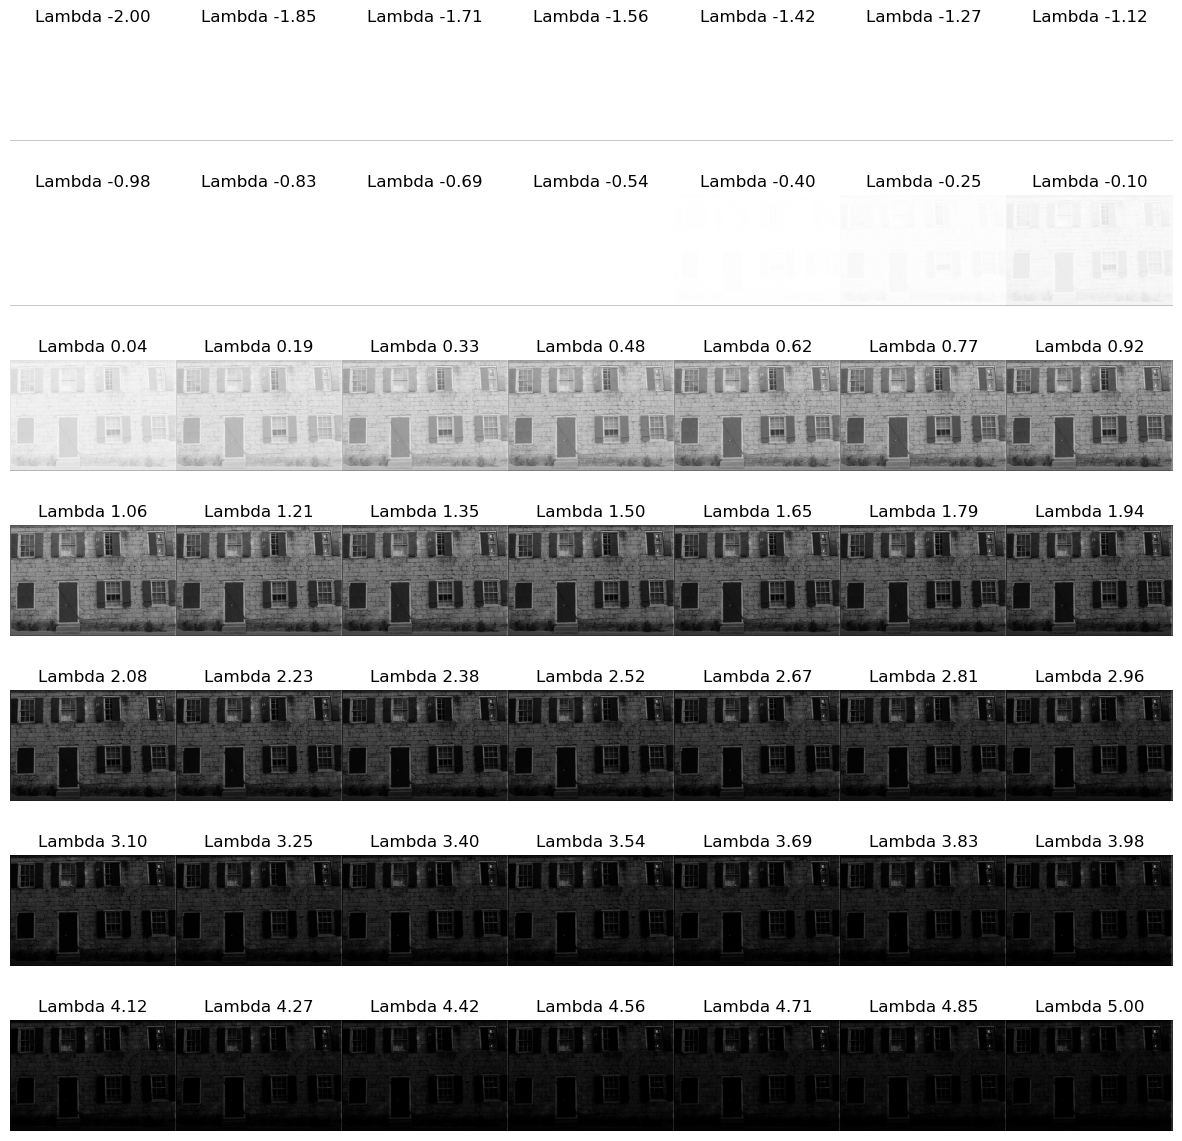
\includegraphics[width=\textwidth]{all_lambda_1.png}
        \caption{Transformaciones de la im\'agen 1.}
        \label{fig:all_lambda_1}
    \end{figure}

    \begin{figure}[H]
        \centering
        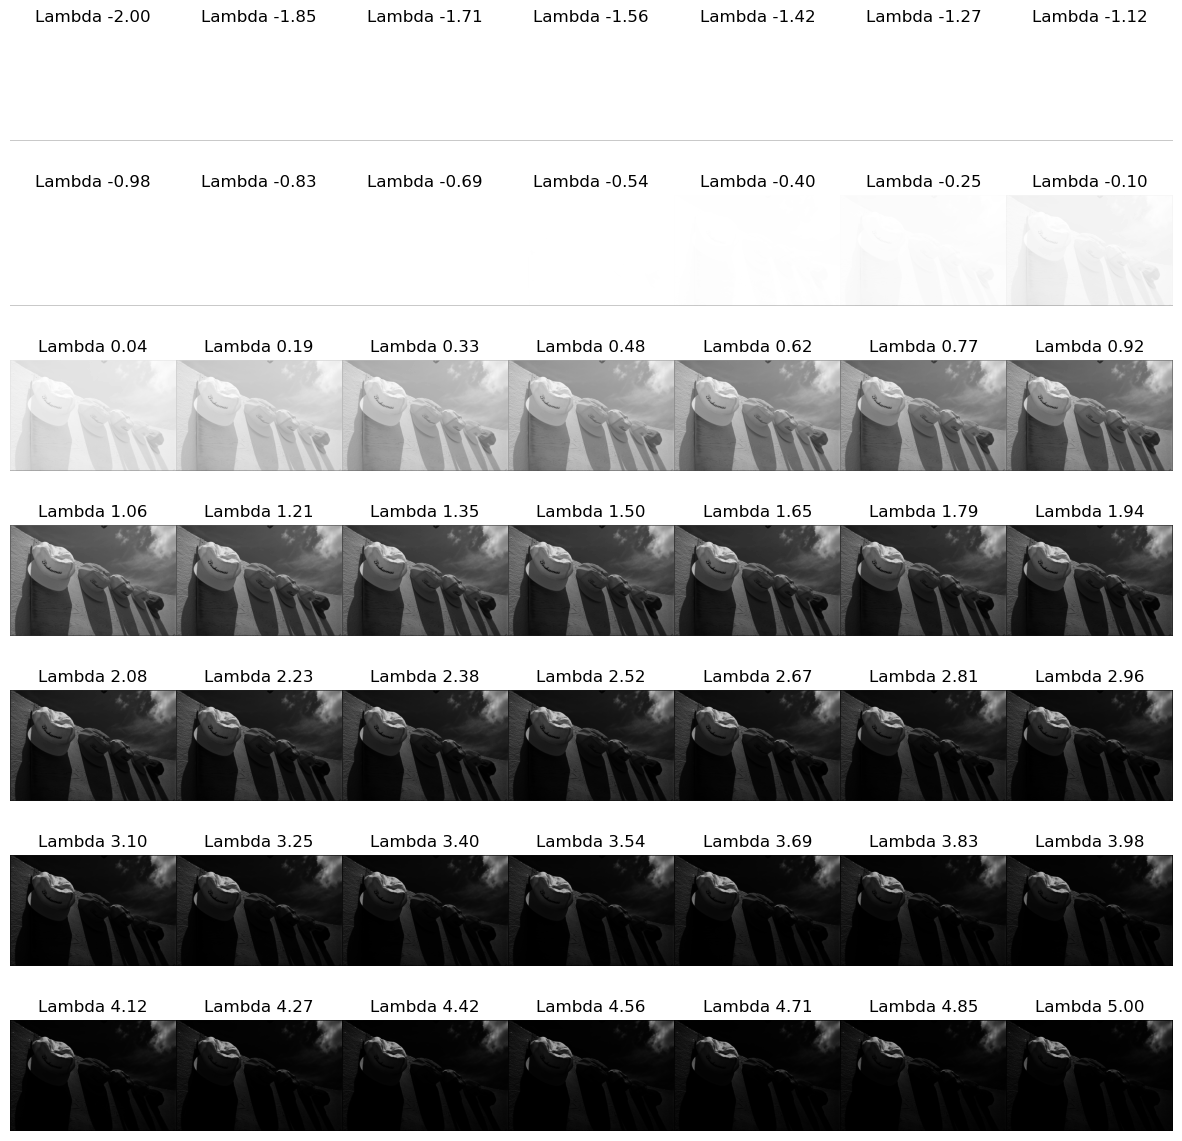
\includegraphics[width=\textwidth]{all_lambda_3.png}
        \caption{Transformaciones de la im\'agen 2.}
        \label{fig:all_lambda_1}
    \end{figure}

    Es claro que, valores m\'as bajos de lambda producen imagenes m\'as claras, hasta el punto en que la imagen es completamente blanca. Por otro lado, valores m\'as altos de lambda producen imagenes m\'as oscuras, pero en general podemos ver que el rango \'util para im\'agenes es $[0,4]$, puesto que valores m\'as altos o m\'as bajos producen imagenes que no son de utilidad. Esto es f\'acil de corroborar al momento de analizar los histogramas. 

    \begin{figure}[H]
        \centering
        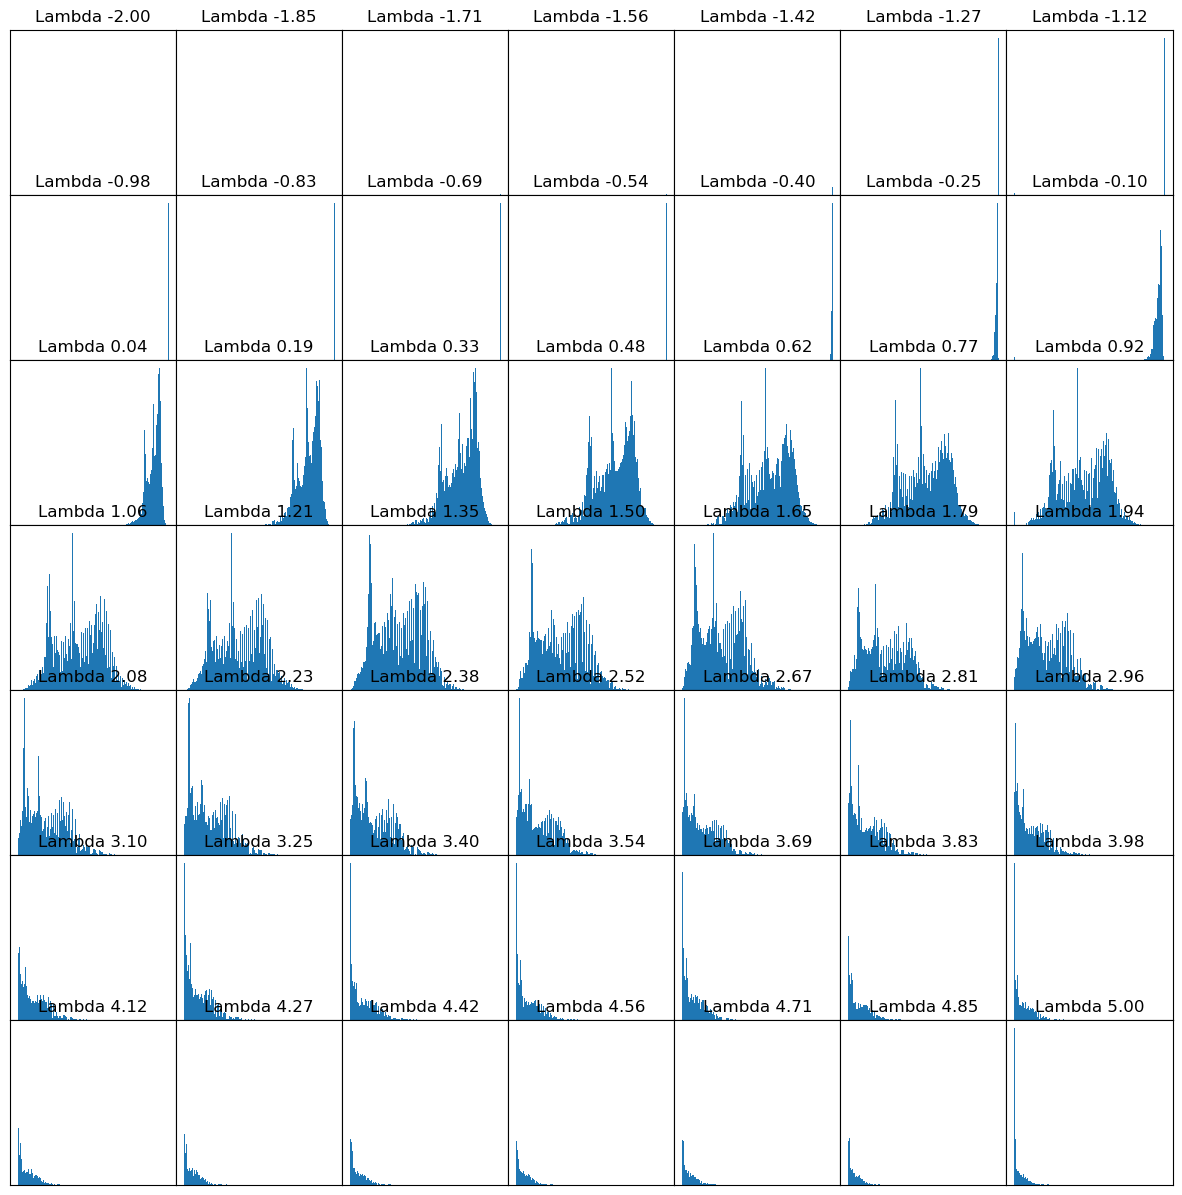
\includegraphics[width=\textwidth]{all_lambda_hist_1.png}
        \caption{Histograma de las transformaciones de la im\'agen 1.}
        \label{fig:img_bci_hist_1}
    \end{figure}

    \begin{figure}[H]
        \centering
        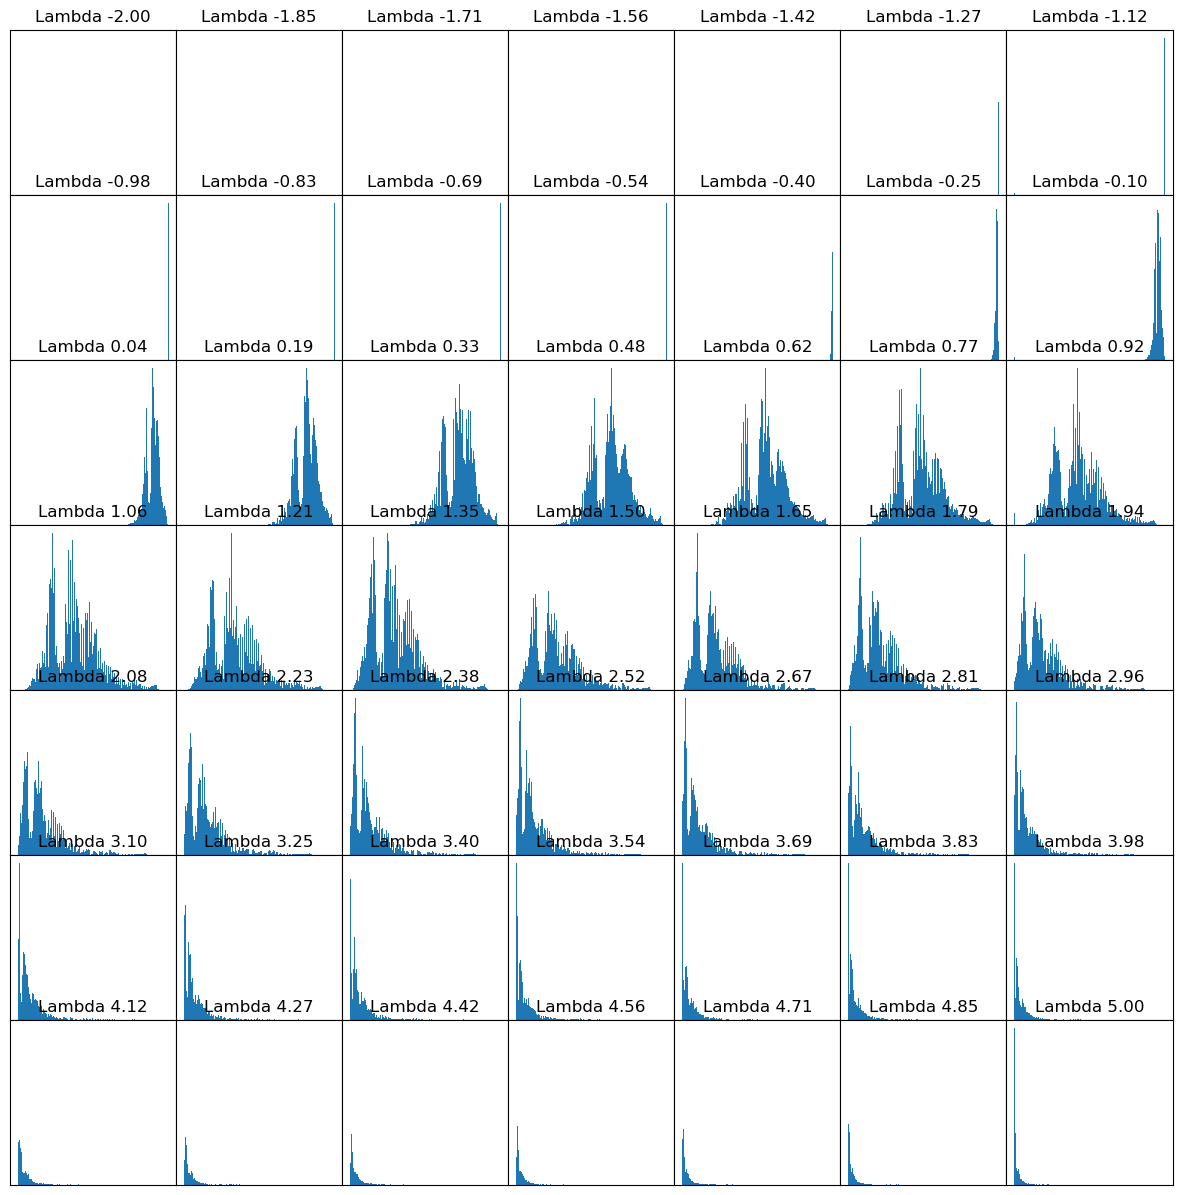
\includegraphics[width=\textwidth]{all_lambda_hist_3.png}
        \caption{Histograma de las transformaciones de la im\'agen 2.}
        \label{fig:img_bci_hist_2}
    \end{figure}
    Podemos ver como la transformacion ''mueve'' los datos hac\'ia la izquierda mientras m\'as alto es el valor de $\lambda$, adem\'as mientras m\'as extremo es este valor, los datos se ven m\'as comprimidos.  

   

    \section[comparando lambdas]{Comparando $\lambda$'s}

    Como mencionamos en la secci\'on anterior, usaremos las im\'agenes mencionadas, ahora en las siguientes figuras \ref{fig:img_bci_1} \ref{fig:img_bci_2} \ref{fig:img_bci_13} \ref{fig:img_bci_22} podemos ver las transformaciones de cada una de est\'as imagenes, junto con el $\lambda$ seleccionado para cada una.

    \begin{figure}[H]
        \centering
        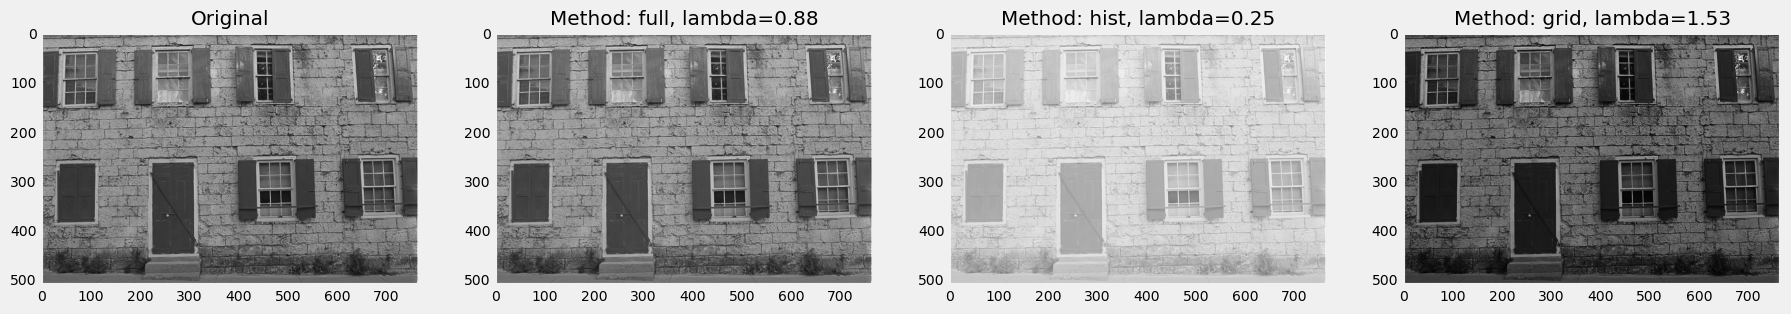
\includegraphics[width=0.9\textwidth]{img_bci_1.png}
        \caption{Transformaciones de la im\'agen 1.}
        \label{fig:img_bci_1}
    \end{figure}

    \begin{figure}[H]
        \centering
        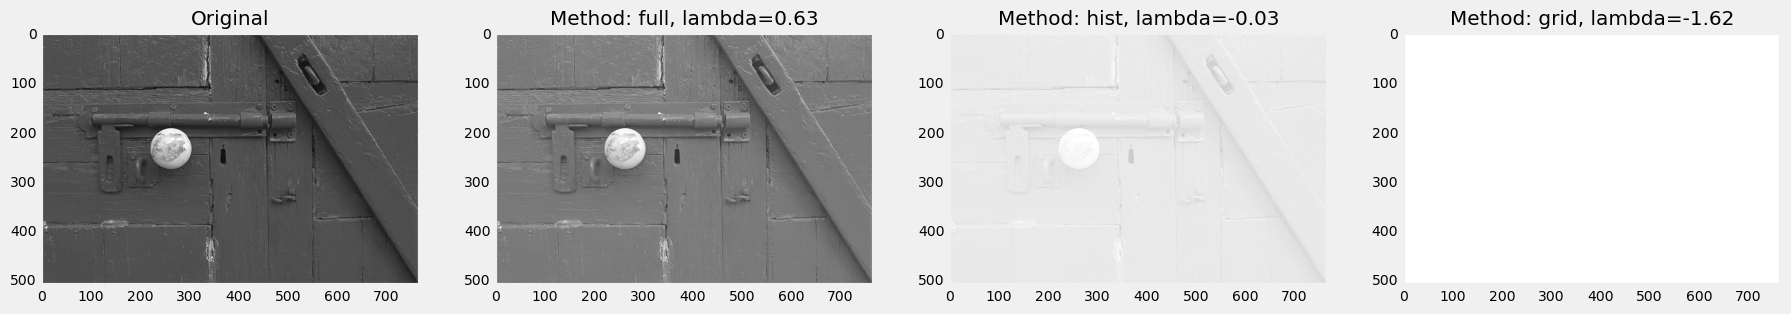
\includegraphics[width=0.9\textwidth]{img_bci_2.png}
        \caption{Transformaciones de la im\'agen 2.}
        \label{fig:img_bci_2}
    \end{figure}

    \begin{figure}[H]
        \centering
        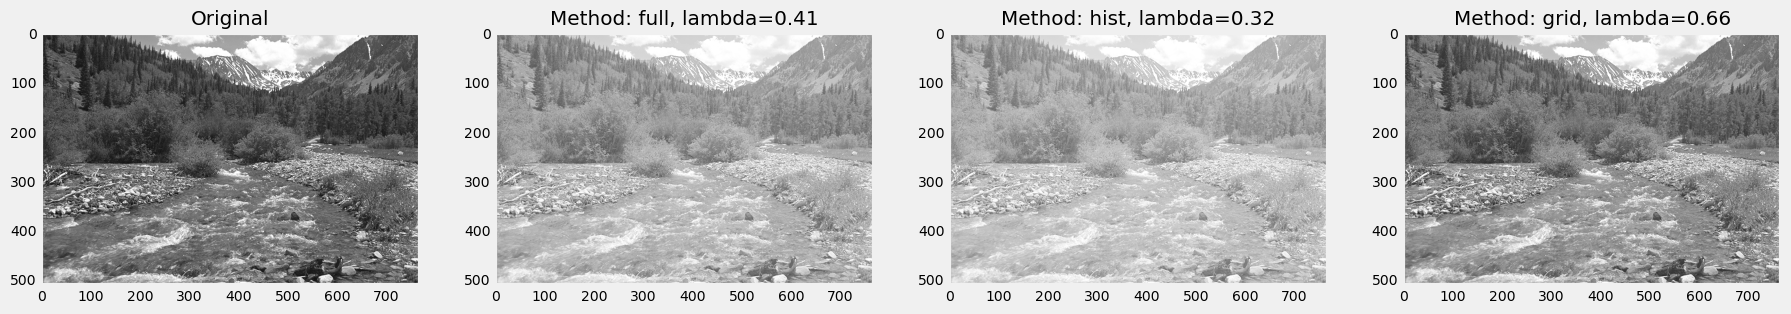
\includegraphics[width=0.9\textwidth]{img_bci_13.png}
        \caption{Transformaciones de la im\'agen 13.}
        \label{fig:img_bci_13}
    \end{figure}

    \begin{figure}[H]
        \centering
        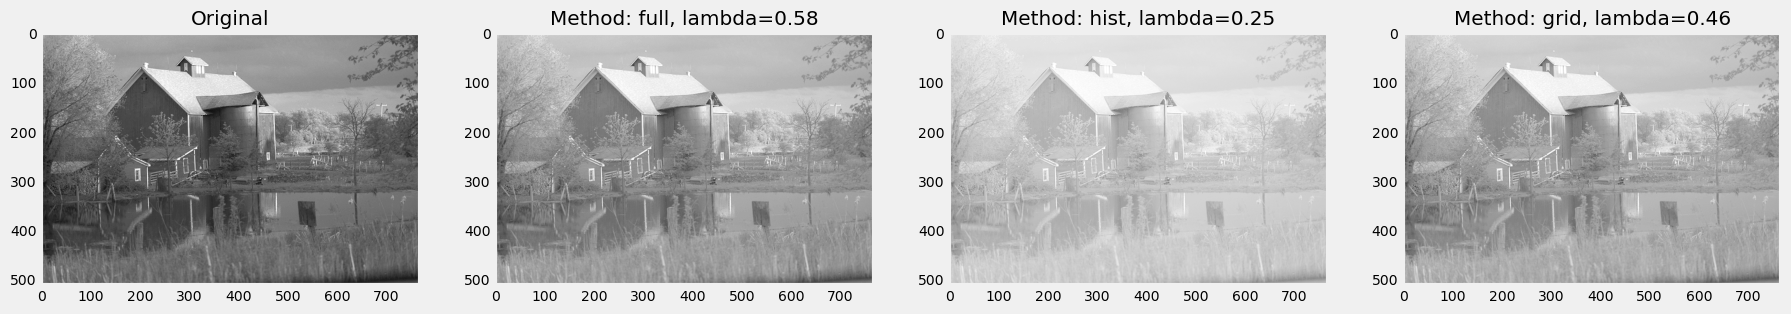
\includegraphics[width=0.9\textwidth]{img_bci_22.png}
        \caption{Transformaciones de la im\'agen 22.}
        \label{fig:img_bci_22}
    \end{figure}

    \todo{juntar imagenes una figura? }

    Lo primero que podemos notar es que el efecto visual que genera cada una de las transformaciones es distinto, \todo{hablar de esto y de las imagenes}. 
    
    No es extra\~no que la composici\'on de cada im\'agen afecta el valor de $\lambda$ seleccionado \todo{hablar cualitaivamente de el efecto que cada forma de transformacion tiene en la imagen}

    \todo{el resto de las iamgenes est\'an en el anexo}

    Ahora, veamos como se comportan $\lambda$ en todo el banco de imagenes.

    \begin{figure}[H]
        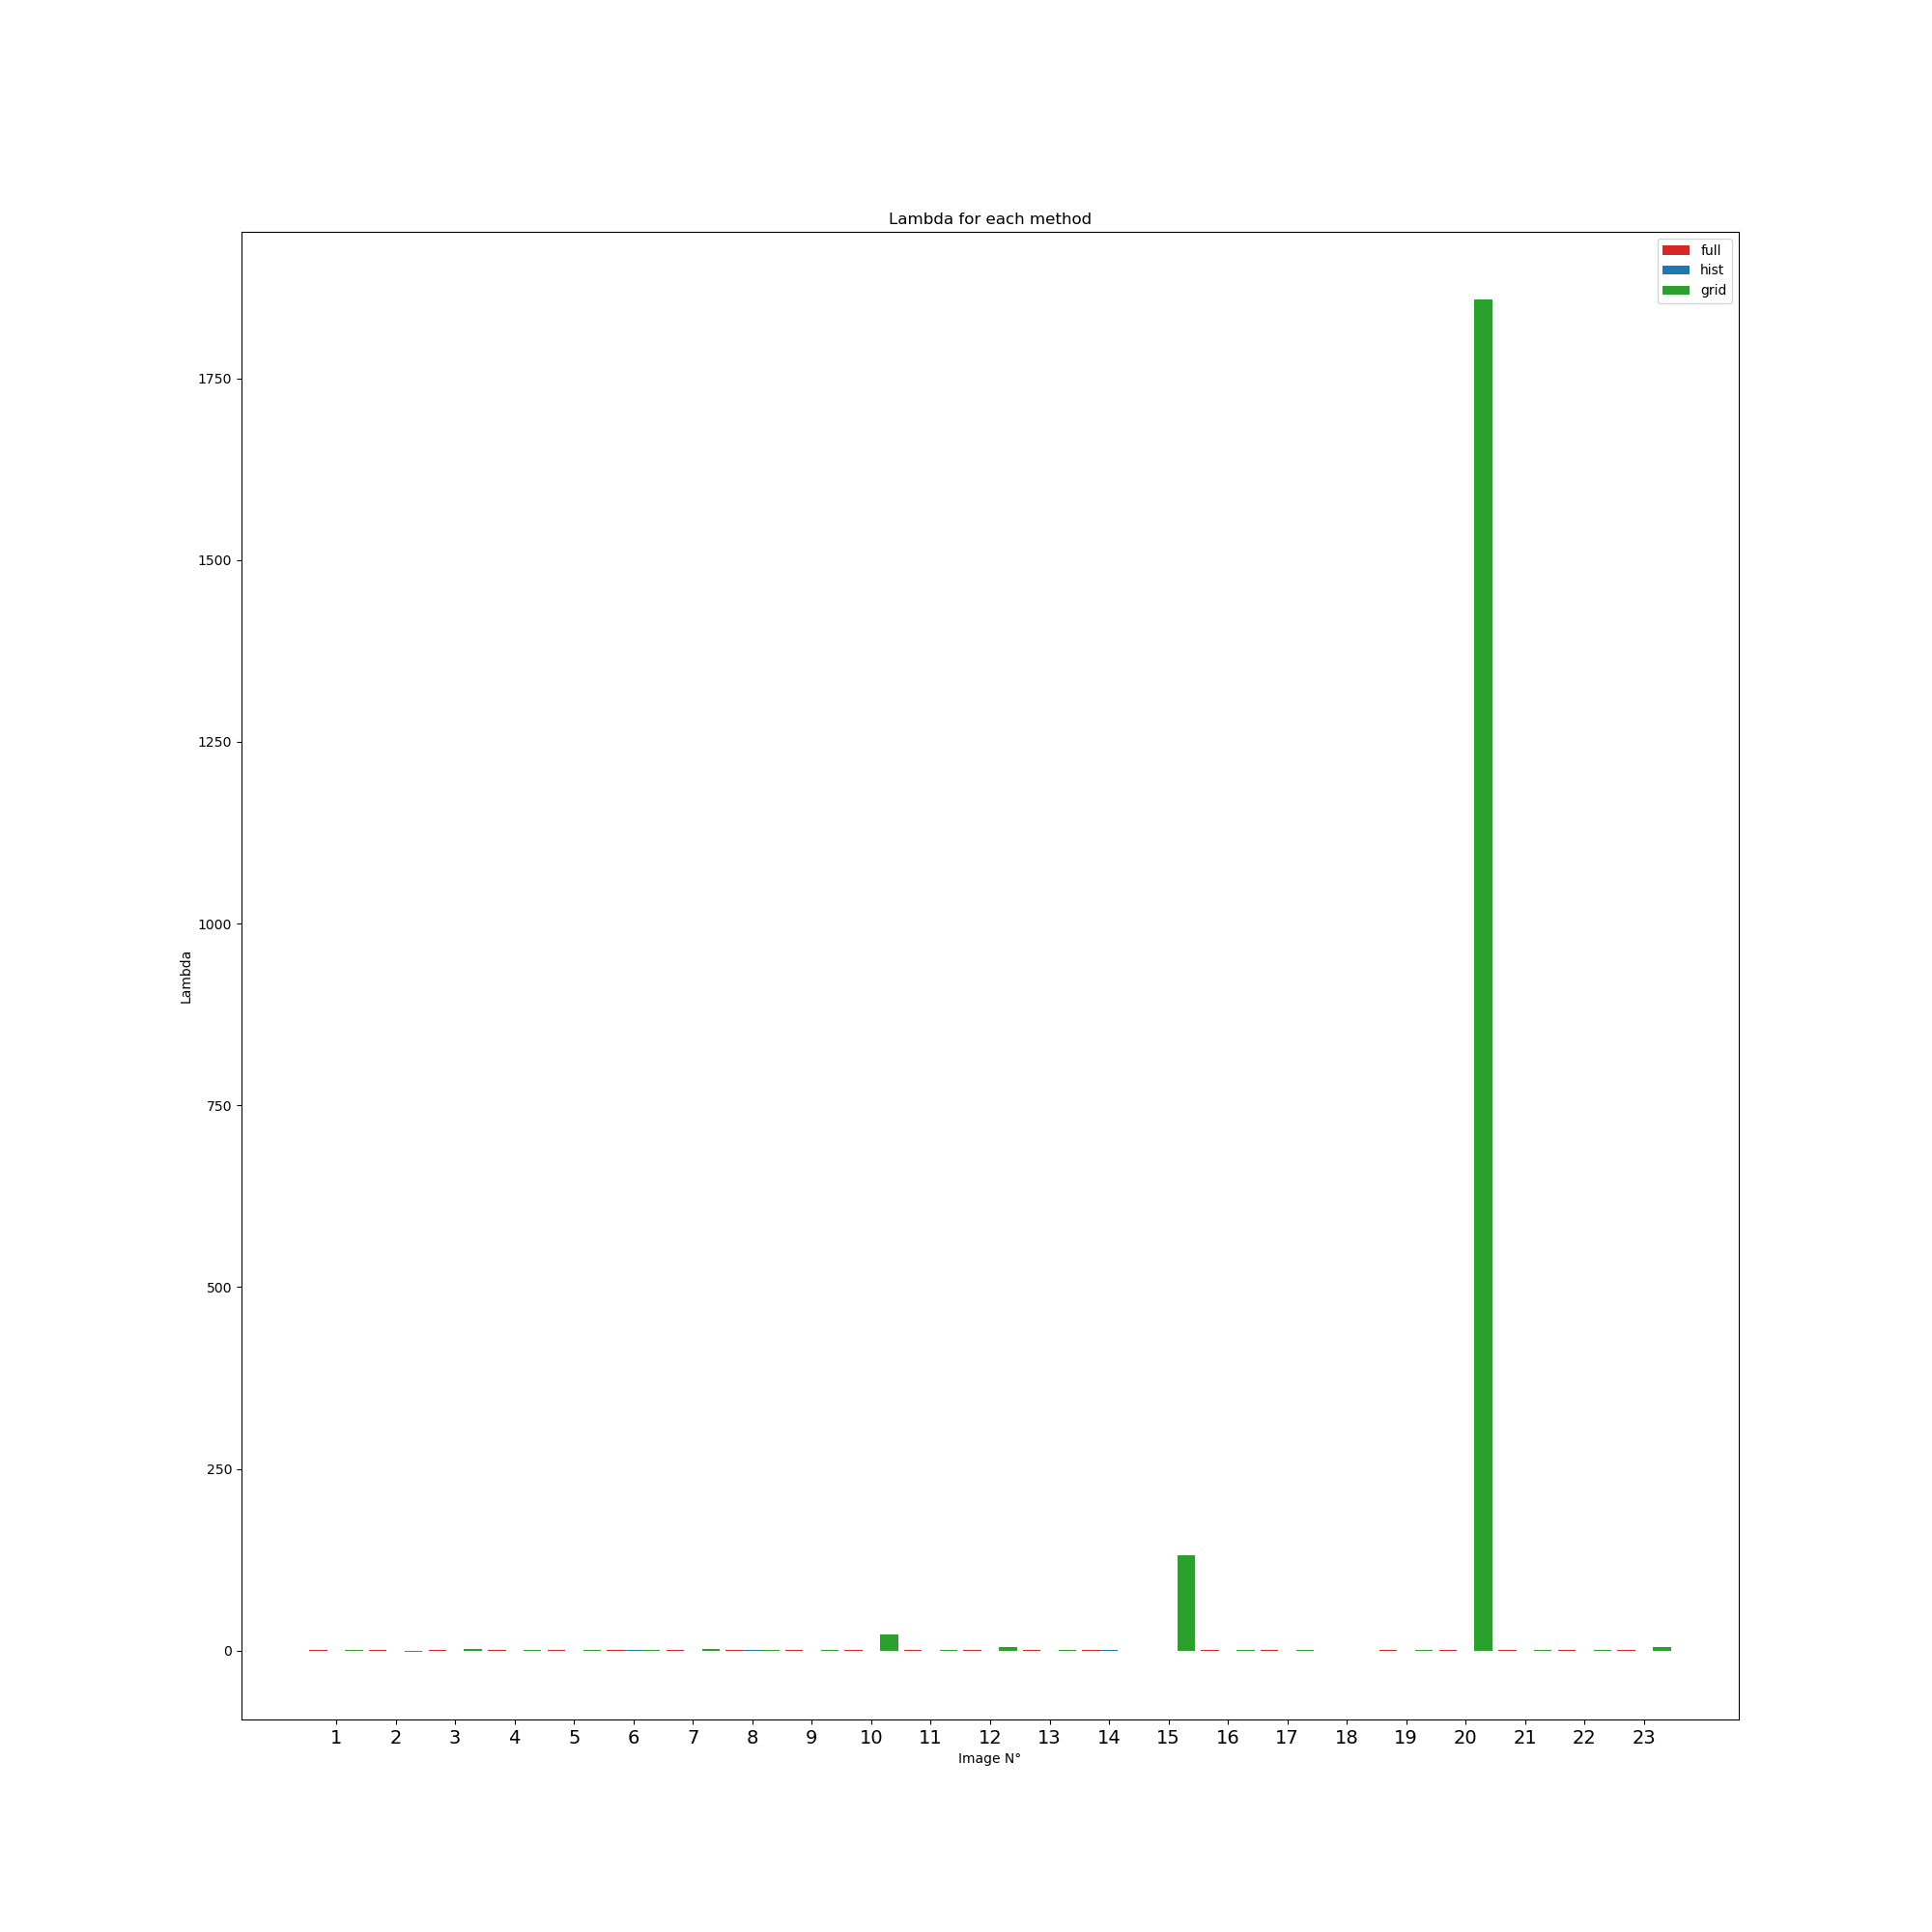
\includegraphics[width=\textwidth]{lambda_noclip.png}
        \caption{Valores de lambda para todo el banco de imagenes. Amarillo es el m\'etodo de grilla, azul es el m\'etodo de histograma, y rojo es el m\'etodo de datos completos}
        \label{fig:lambda_noclip}
    \end{figure}

    \todo{Podemos ver que en elgunos casos lamba se demasiado solo pasa en gris}. Notemos que las im\'agenes cuyo $\lambda$ se dispara son las imagenes 10, 15, y 20, las cuales podemos ver a continuaci\'on en la figura \ref{fig:img_bci_10_15_20}

    \begin{figure}[H]
        \centering
        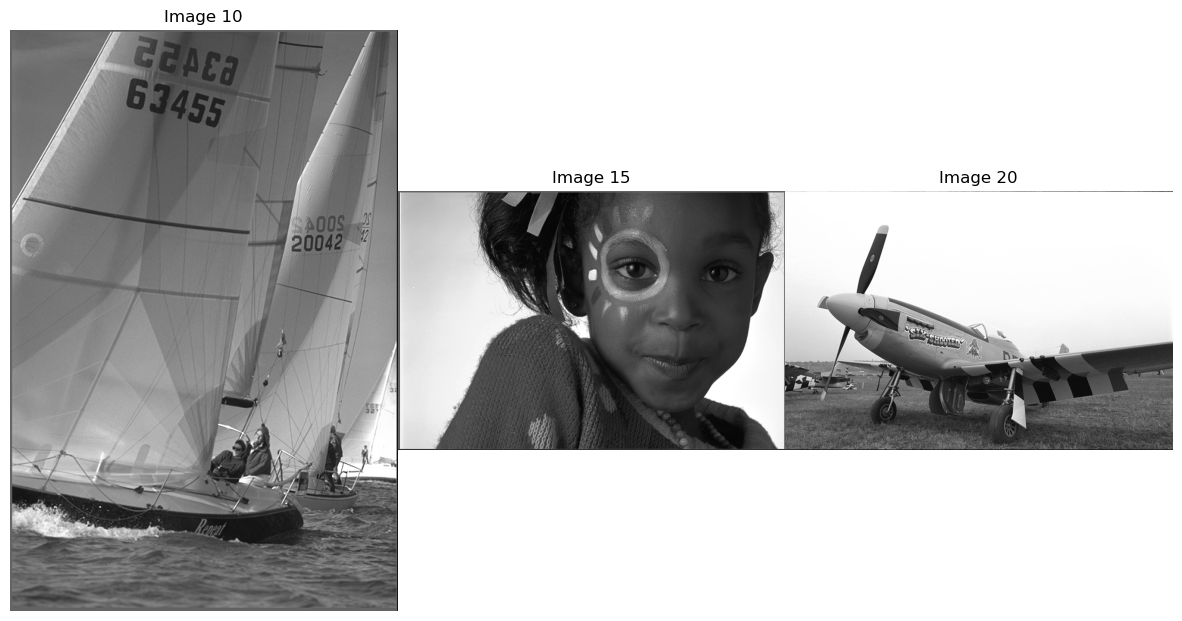
\includegraphics[width=0.9\textwidth]{img_ex_10_15_20.png}
        \caption{Transformaciones de las imagenes 10, 15, y 20.}
        \label{fig:img_bci_10_15_20}
    \end{figure}

    Lo que est\'as imagenes tienen en com\'un es que son im\'agenes que contienen grandes secciones de color similar, lo que genera al momento de hacer la grilla, que muchas secciones se ven ''planas'', esto genera que el valor de $\lambda$ se dispare. Ahora, vamos a cortar los valores en $5$ para poder ver mejor el comportamiento de $\lambda$ en el resto de las imagenes.

    \begin{figure}[H]
        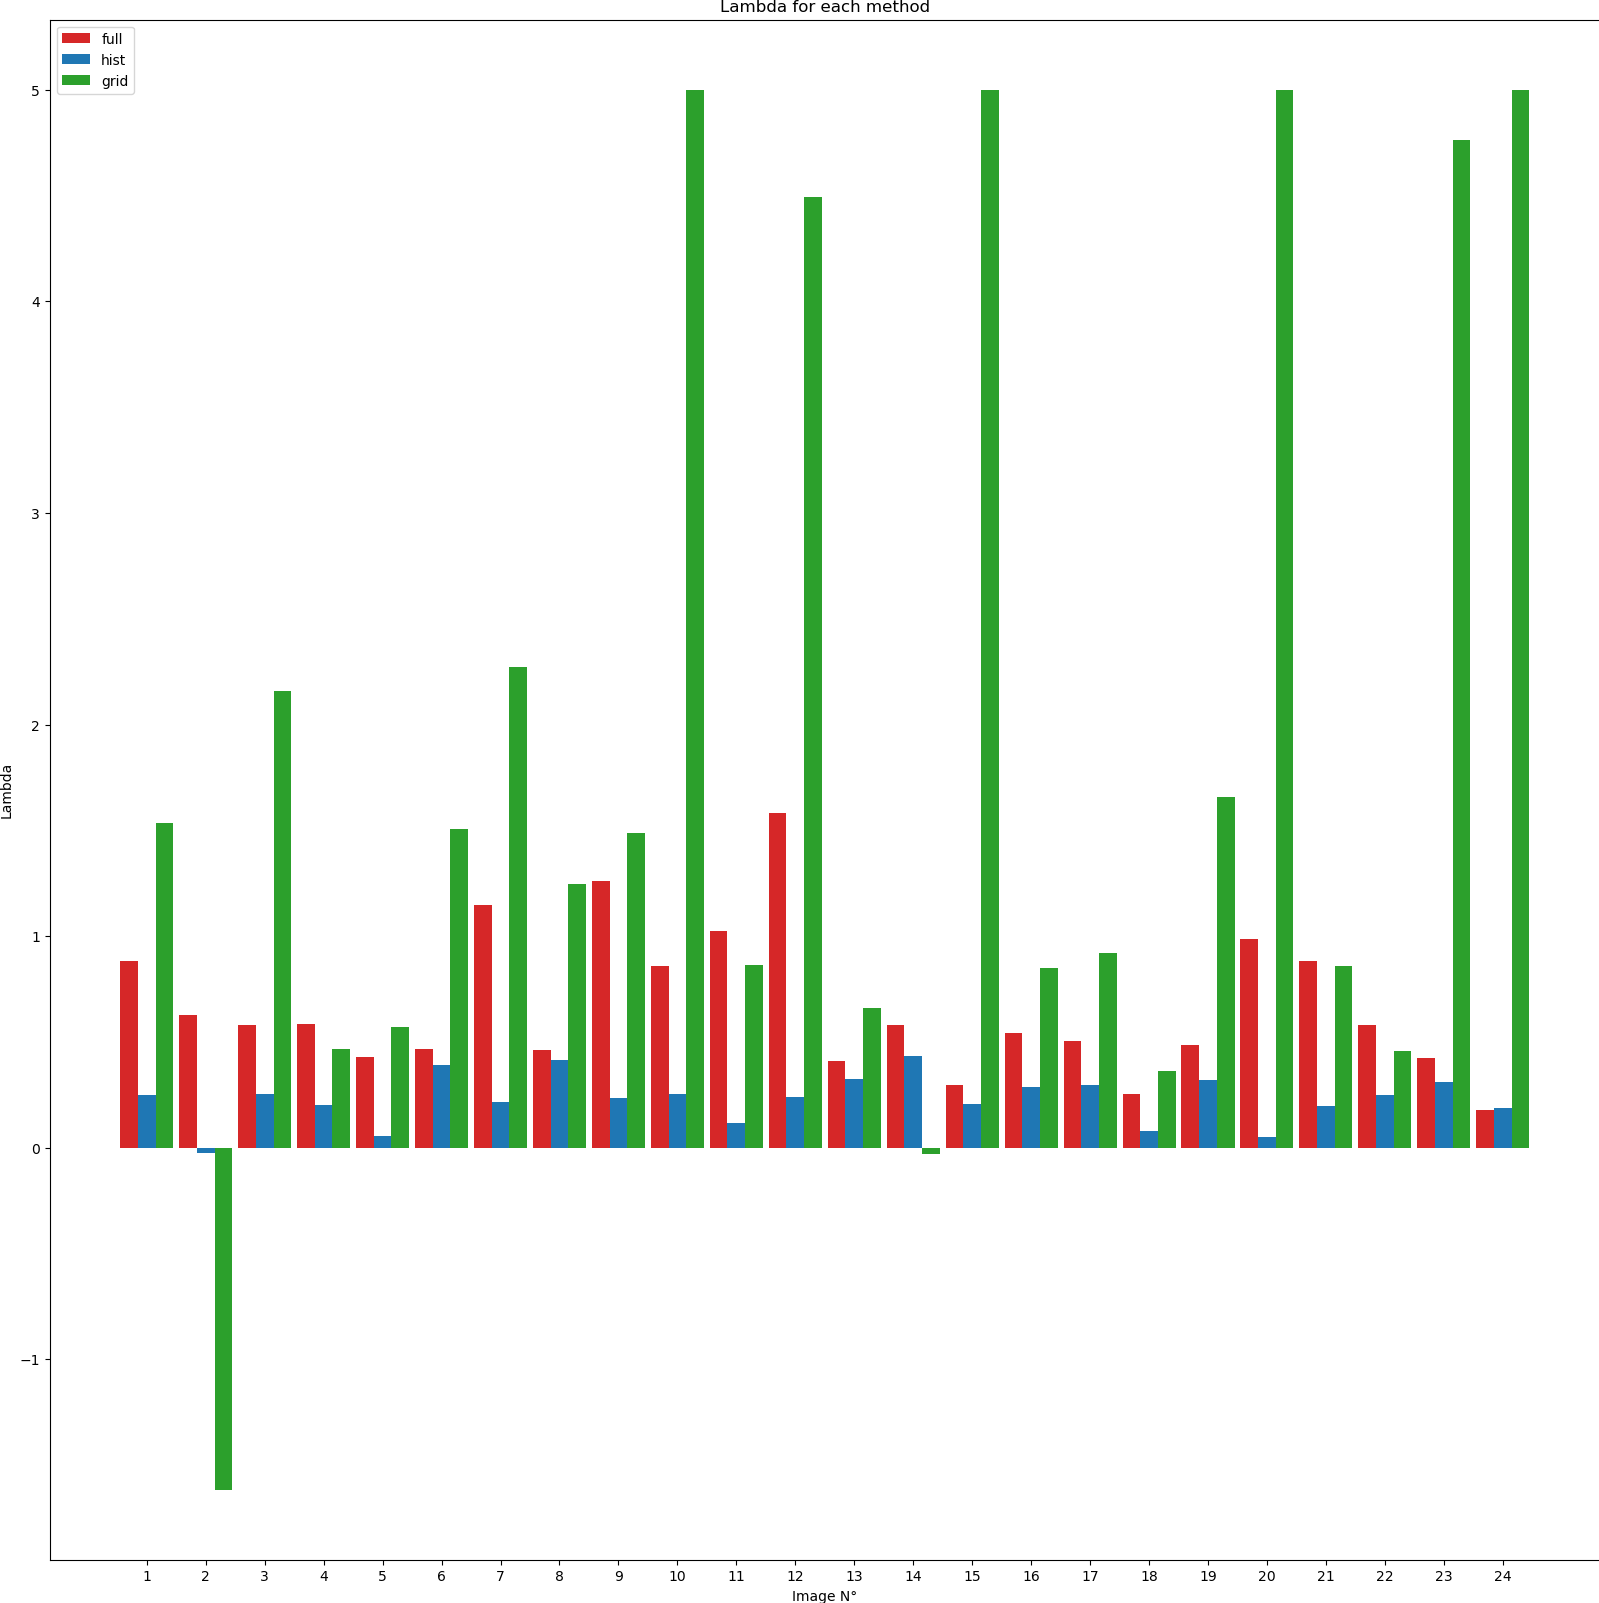
\includegraphics[width=\textwidth]{lambda_clip.png}
        \caption{Valores de lambda para todo el banco de imagenes, cortado en 5. Amarillo es el m\'etodo de grilla, azul es el m\'etodo de histograma, y rojo es el m\'etodo de datos completos}
        \label{fig:lambda_clip}
    \end{figure}

   \todo{ podemos ver que esto, hablar de correlaciones entre los valores de lambda, y como se comportan en distintos tipos de imagenes.}


   resultado de las correlaciones de pearson entre los distintos metodos de seleccion de lambda

    full, hist PearsonRResult(r=-0.1621, pvalue=0.4598)

    full, grid PearsonRResult(r=0.1785, pvalue=0.4149)

    hist, grid PearsonRResult(r=-0.3417, pvalue=0.1105)

    \todo{hablar de esto}

    \section{Box-Cox sobre imagenes a color}

    A pesar de que en este trabajo nos centrados en discutir la transformaci\'on de Box-Cox sobre imagenes en escala de grises, vale la pena mencionar es posible extender la transformaci\'on a imagenes a color. Para esto podemos encontrar un lambda para cada canal de color, y luego aplicar la transformaci\'on sobre cada canal, o podemos aplicar la transformaci\'on sobre cada color de la im\'agen. 


    En la figura podemos ver algunos ejemplos de la primera transformaci\'on descrita. \todo{hacer imagen} No ahondaremos m\'as en este concepto cabe mencionar este fue el m\'etodo usado por Cheddad \cite{boxcoximg} en su trabajo.

    \section{Concluciones}